 % Write the body to be read by cstwMPC-Slides-Print.tex for autogeneration of printable version
\usepackage{cancel}
\usepackage{econtexShortcuts}
%\newcommand*{\newblock}{} % Needed to make beamer work with bibtex

\pdfmapfile{+sansmathaccent.map}
% Jirka's definitions
\usepackage{booktabs, natbib}
\definecolor{jirkasred}{rgb}{0.9,0,0}
\newcommand{\jemph}[1]{{\color{jirkasred}#1}}
%\def\newblock{\hskip .11em plus .33em minus .07em}

\renewcommand{\ptyLev}{\ensuremath{Z}} % Z for productivity
\renewcommand{\urate}{\ensuremath{u}}
\renewcommand{\erate}{\ensuremath{\cancel{\urate}}}

%\setbeamertemplate{navigation symbols}{}  % Take away navigation symbols

%_____________ Opening slide _______________________

\title[Wealth and MPC]{{The Distribution of Wealth and \\ the Marginal Propensity to Consume}}
\author[Carroll, Slacalek, Tokuoka and White]{\scriptsize{Christopher Carroll\inst{1} \and Jiri Slacalek\inst{2} \and Kiichi Tokuoka\inst{3} \and Matthew N. White\inst{4}}}

% - Use the \inst command only if there are several affiliations.
% - Keep it simple, no one is interested in your street address.
\institute{
  \inst{1} Johns Hopkins University and NBER\\   \texttt{ccarroll@jhu.edu} \and
  \inst{2} European Central Bank\\   \texttt{jiri.slacalek@ecb.int} \and
  \inst{3} Ministry of Finance, Japan\\   \texttt{kiichi.tokuoka@mof.go.jp} \and
  \inst{4} University of Delaware\\   \texttt{mnwecon@udel.edu}
    }
%\date{Vancouver, July 2013}
\date{}

\begin{document}

\begin{frame}[plain]
  \titlepage
\end{frame}



\section{Motivation}

\subsection{The MPC}

\input ./Individual/OurClaim.tex



\subsection{Theory and Evidence}
\begin{frame}[label=cFuncAndW]
\frametitle{Consumption Concavity and Wealth Heterogeneity}
\begin{figure}
\centering
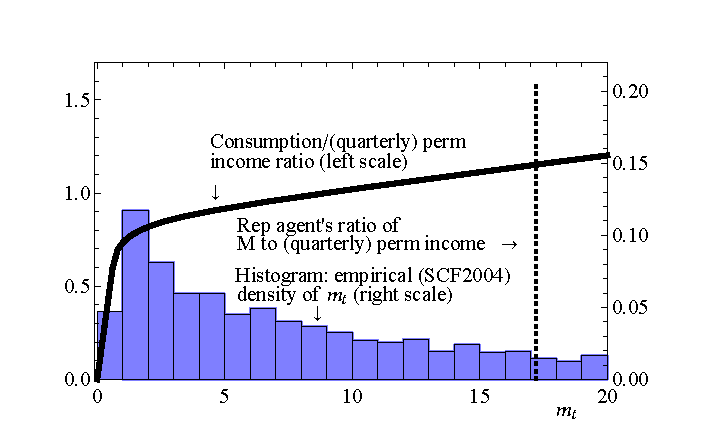
\includegraphics[width=\textwidth,height=6.3cm]{../Figures/CFuncPointAndHistNetWorthPlot.pdf}
\end{figure}
\end{frame}


\input ./Individual/WhyWorryAboutMPC.tex

\begin{comment}
%_____________ 1st section  ____________
\subsection{Essential Consumption Microfoundations}
\begin{frame}
\frametitle{Microeconomics of Consumption}

\begin{block}{Since Friedman's (1957) PIH:}
  \begin{itemize}
    \item $c$ chosen optimally:\\
     \jemph{~~Want to smooth $c$ {\it in light of} $y$ fluctuations}
    \item Single most important thing to get right is \jemph{{income dynamics}}!
    \item With smooth $c$, income dynamics \jemph{drive everything!}
    \begin{itemize}
        \item \jemph{Saving/dissaving:} Depends on whether $\Ex[\Delta y]\uparrow$ or $\Ex[\Delta y]\downarrow$
        \item \jemph{Wealth distribution} depends on integration of saving
    \end{itemize}
    \item \jemph{Cardinal sin:} Assume crazy income dynamics
    \begin{itemize}
      \item No end can justify this means
      \item Throws out the defining core of the intellectual framework
    \end{itemize}
  \end{itemize}
\end{block}

\end{frame}

\end{document}

\begin{frame}
\frametitle{Our Goal: ``Serious'' Microfoundations}

Requires three changes to well-known \jemph{Krusell--Smith (1998)} model: \pause
\begin{enumerate}
\item Sensible microeconomic income process: Friedman
\item Finite lifetimes: Blanchard
\item Match wealth \jemph{distribution}
\bi
\item Here, achieved by preference heterogeneity
\item View it as a proxy for many kinds of heterogeneity
\bi
\item Age
\item Growth
\item Risk aversion
\item \dots
\ei
\ei
\end{enumerate}
\end{frame}
\end{comment}




\begin{frame}
\frametitle{{To-Do List}}


\begin{enumerate}
\item Calibrate realistic income process
\item Match empirical wealth distribution
\item Back out optimal C and MPC out of transitory income
\item Is MPC in line with empirical estimates?
\end{enumerate}


\begin{block}{Our Question:}
\jemph{Does a model that matches micro facts} about income dynamics and wealth distribution \jemph{give different} (and more plausible) \jemph{answers} than KS \jemph{to macroeconomic questions} (say, about the response of consumption to fiscal `stimulus')?
\end{block}
\end{frame}


%_______________________________________
\subsection{Friedman (1957)}
\begin{frame}
\frametitle{{\citet{friedmanAtheory}: Permanent Income Hypothesis}}
\begin{eqnarray*}
Y_{t}&=&P_{t}+T_{t}\\
C_{t}&=&P_{t}
\end{eqnarray*}

\begin{block}{Progress since then}
\begin{itemize}
  \item \jemph{Micro data:} Friedman description of income shocks works well
  \item \jemph{Math:} Friedman's words well describe optimal solution to dynamic stochastic optimization problem of impatient consumers with geometric discounting under CRRA utility with uninsurable idiosyncratic risk calibrated using these micro income dynamics (\jemph{!})
\end{itemize}
\end{block}

\end{frame}

\begin{comment} % Already said this above
%_______________________________________
\subsection{Modifications to the Benchmark KS model}
\begin{frame}
\frametitle{{Use the Benchmark KS model with Modifications}}



\begin{block}{Modifications to \citet{ksHetero}}
  \begin{enumerate}
    \item Serious \jemph{income process}
        \begin{itemize}
        \item MaCurdy, Card, Abowd; Blundell, Low, Meghir, Pistaferri, \dots
        \end{itemize}
    \item \jemph{Finite lifetimes} (i.e., introduce \citet{blanchard:finite} death, $\PDies$)
    \item Heterogeneity in \jemph{time preference factors}
  \end{enumerate}
\end{block}

\end{frame}

\end{comment}

\section{Model Without Aggregate Shock}

%_______________________________________
\subsection{Income Process}
\begin{frame}
\frametitle{{Our (Micro) Income Process}}

Idiosyncratic (household) income process is logarithmic Friedman:
  \begin{eqnarray*}
\yLev_{t+1}&=&\pRat_{t+1}\tshk_{t+1}\Wage\\
\pRat_{t+1}&=&\pRat_{t}\pshk_{t+1}
\end{eqnarray*}
$\pRat_{t}=$ permanent income\\
$\tshk_{t}=$ transitory income\\
$\pshk_{t+1}=$ permanent shock\\
$\Wage=$ aggregate wage rate
\end{frame}

\begin{frame}
\frametitle{{Further Details of Income Process}}

\begin{block}{Modifications from \citet{carroll:brookings}}
Transitory income $\tshk_{t}$ incorporates \jemph{unemployment insurance}:
\begin{eqnarray*}
\tshk_{t} &=&\mu \text{ with probability $u$} \\
&=&(1-\tau)\bar{\ell}\theta_{t}\text{ with probability $1-u$}
\end{eqnarray*}
$\mu$ is UI when unemployed\\
 $\tau$ is the rate of tax collected for the unemployment benefits
\end{block}

\end{frame}


%_______________________________________
\subsection{Decision Problem}
\begin{frame}
\frametitle{{Model Without Aggr Uncertainty: Decision Problem}}

\providecommand{\util}{u}

\begin{eqnarray*}
\valfn(\mRat_{t})&=& \underset{\{\cFunc_{t}\}}{\max } ~~
\util%(\cRat_{t})
+\Discount \PLives \Ex_{t}\left[ \pshk_{t+1}^{1-\CRRA}\valfn(\mRat_{t+1})
\right]   \label{eq:hetdecisionprobnashk}\\
\notag &\text{s.t.}&\\
\notag \wEndRat_{t} &=&\mRat_{t}-\cRat_{t} \\
\notag \wEndRat_{t} &\geq &0 \\
\kRat_{t+1} &=&\wEndRat_{t}/(\PLives \pshk_{t+1})  \label{indconst3}
\\
\mRat_{t+1} &=&(\daleth +\rProd)\kRat_{t+1}+\tshk_{t+1} \label{indconst4} \\
\notag \rProd &=&\kapShare\ptyLev(\KLev/\bar{\ell}\LLev)^{\kapShare-1}
\end{eqnarray*}
(State and control variables normalized by $\pRat_{t} \Wage$)

\end{frame}


%_______________________________________
%\subsection{What Happens After Death?}
\subsection{There Is an Ergodic Distribution of Permanent Income}
\begin{frame}
\frametitle{{What Happens After Death?}}

\pause
\begin{itemize}
\item You are replaced by a new agent whose permanent income is equal to the population mean
\item Prevents the population distribution of permanent income from spreading out
\end{itemize}
\end{frame}


%_______________________________________
%\subsection{There Is an Ergodic Distribution of Permanent Income}
\begin{frame}
\frametitle{{Ergodic Distribution of Permanent Income}}

Exists, if death eliminates permanent shocks:
$$\PLives \Ex[\pshk^{2}] < 1.$$
 \jemph{Holds.}\\[5mm]
Population mean of $\pRat^{2}$:
\begin{eqnarray}
\Mean[\pRat^{2}] & = & \frac{\PDies}{1-\PLives\Ex[\pshk^{2}]}\notag
\end{eqnarray}

\end{frame}

%_______________________________________
\subsection{Parameter Values}
\begin{frame}
\frametitle{{Parameter Values}}
\begin{itemize}
  \item $\beta $, $\CRRA $, $\kapShare $, $\delta $, $\bar{\ell}$, $\mu$ , and $u$ taken from JEDC special volume %(from \citet{denhann:comp})
  \item Key new parameter values:
\end{itemize}

  \begin{footnotesize}
  \begin{table}
  %\caption{Parameter Values}

  \begin{center}
  \begin{tabular}{cccc}
  \toprule
  Description              & Param       & Value   & Source\\ \midrule
  Prob of Death per Quarter& $\PDies$        & $0.00625$ & Life span of 40 years\\
  Variance of Log $\pshk_{t}$ & $\sigma _{\pshk}^{2}$ & $0.016/4$ &\text{\small{\citet{carroll:brookings}}}; SCF \\
    & & & \text{\small{DeBacker et al.\ (2013)}}\\
  Variance of Log $\theta _{t}$ & $\sigma _{\theta }^{2}$& $0.010\times 4$ & \text{\small{\citet{carroll:brookings}}}\\
 \bottomrule
  \end{tabular}
  \end{center}
  \end{table}
  \end{footnotesize}

\end{frame}



%_______________________________________
\subsection{Annual Income Variances}
\begin{frame}
\frametitle{{Annual Income, Earnings, or Wage Variances}}

\begin{scriptsize}
\input ../Tables/EstimatesOfVarsslides.tex

\tiny{$^{\star}$\citet{meghir&pistaferri} and \citet{bppInequality} assume that the transitory component is serially correlated (an MA process), and report the variance of a subelement of the transitory component. $\sigma_{\tshk}^{2}$ for these articles are calculated using their MA estimates. }
\end{scriptsize}

\end{frame}



%_______________________________________
\subsection{Estimation/Results}


%_______________________________________
\subsection{Our Strategy}
%\begin{frame}
%\frametitle{{Our Strategy}}
%\begin{enumerate}
%  \item Estimate the time preference factor $\beta$ without aggregate shock
%  \item Using estimated $\beta$, run model(s) with aggregate shocks
%\end{enumerate}
%\end{frame}



\begin{frame}
\frametitle{{Typology of Our Models---{Four Dimensions}}}

\begin{block}{}\footnotesize
\begin{enumerate}
\item \jemph{Discount Factor $\Discount$}
\bi \scriptsize
\item \jemph{`$\Discount$-Point' model:} Single discount factor
\item \jemph{`$\Discount$-Dist' model:} Uniformly distributed discount factor
\ei
\item \jemph{Aggregate Shocks}
\bi \scriptsize
\item (No)
\item Krusell--Smith
\item Friedman/Buffer Stock
\ei
\item \jemph{Empirical Wealth Variable to Match}
\bi \scriptsize
\item Net Worth
\item Liquid Financial Assets
\ei
\item \jemph{Life Cycle}
\bi \scriptsize
\item Perpetual Youth (a la Blanchard)
\item Overlapping Generations
\ei
\end{enumerate}
\end{block}

\end{frame}


\begin{frame}
\frametitle{{Dimension 1: Estimation of $\Discount$-Point and $\Discount$-Dist}}

\begin{footnotesize}
\begin{block}{`$\Discount$-Point' model}
\bi
\item `Estimate' single $\grave{\Discount}$ by matching the capital--output ratio
\ei
\end{block}
\begin{block}{`$\Discount$-Dist' model---Heterogenous Impatience}
\begin{itemize}
\item Assume uniformly distributed $\Discount$ across households
%\item Estimate the band $[\grave{\Discount}-\nabla,\grave{\Discount}+\nabla]$ by matching net worth held by the top 20, 40, 60, 80\%
\item Estimate the band $[\grave{\Discount}-\nabla,\grave{\Discount}+\nabla]$ by \jemph{minimizing distance between model ($w$) and data ($\omega$) net worth} held by the top 20, 40, 60, 80\%
%        \item The uniform distribution is approximated by 7 points
       % \item \jemph{Minimize distance b/w model ($w$) and data ($\omega$) wealth quantiles}:
        \begin{equation*}
        \underset{\{\grave{\Discount}, \nabla\}}{\min}\sum\limits_{i=20,40,60,80}(w_{i}-\omega _{i})^{2}\notag,
        \end{equation*}
        s.t. aggregate net worth--output ratio matches the steady-state value from the perfect foresight model\\[2mm]
        %\footnotesize $w_{i}$ and $\omega _{i}$ are proportions of net worth held by the top $i$ percent in our model and in the data, respectively
\end{itemize}
\end{block}
\end{footnotesize}

\end{frame}

%_______________________________________

\begin{frame}
\frametitle{{Results: Wealth Distribution}}

\begin{figure}
\centering
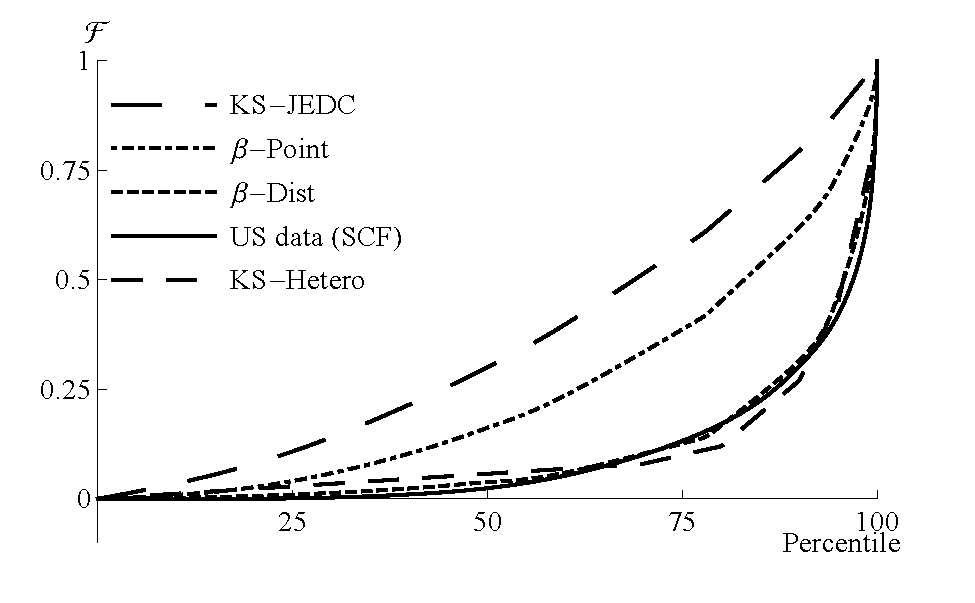
\includegraphics[width=0.9\textwidth]{../Figures/CumWLevSCFCastanedaAndDistSevenNoAggShockPlot.pdf}
%\caption{Cumulative Distribution of Net Worth}
\label{CumWLevSCFCastanedaAndDistSevenNoAggShockPlot}
\end{figure}

\end{frame}



\begin{frame}
\frametitle{{Results: Wealth Distribution}}

\begin{table}
\begin{footnotesize}

\input ../Tables/WDistslides.tex

\end{footnotesize}
\end{table}
\tiny{Notes: $^{\ddagger}:$ $\grave{\Discount}=
\input ../../../cstCode/Latest/Code/Mathematica/Results/Beta.tex
$.
$^{\star}:$ $(\grave{\Discount}, \nabla)=(
\input ../../../cstCode/Latest/Code/Mathematica/Results/Betamiddle.tex
,
\input ../../../cstCode/Latest/Code/Mathematica/Results/nabla.tex
)$%
.
Bold points are targeted. $\KLev_{t}/\YLev_{t}=10.3$. }
\end{frame}

%_______________________________________
\subsection{Results: Marginal Propensity to Consume}

\begin{frame}
\frametitle{{Marginal Propensity to Consume \& Net Worth}}

\begin{figure}
\centering
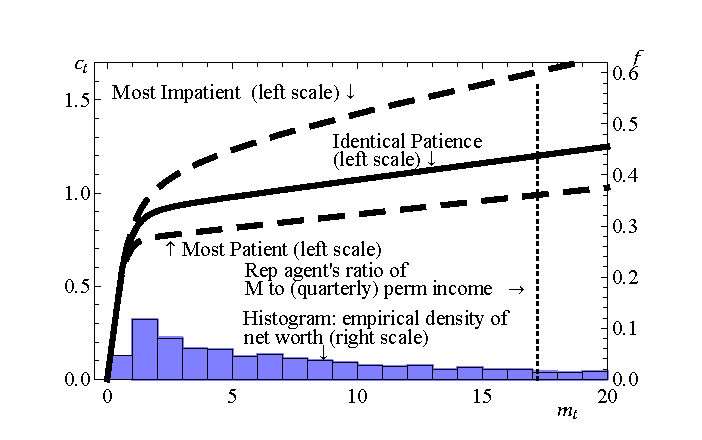
\includegraphics[width=\textwidth,height=6cm]{../Figures/CFuncDistSevenPointPermAndHistNetWorthPlotFedQuarterly.pdf}
\end{figure}

\end{frame}

%_______________________________________
\begin{frame}
\frametitle{{Results: MPC (in Annual Terms)}}
\begin{scriptsize}
\begin{table}
\input ../Tables/MPCslides.tex
\end{table}
\tiny{Notes: Annual MPC is calculated by $1-(1-$\text{quarterly MPC}$)^{4}$.
% See the paper for a discussion of the extensive literature that generally estimates empirical MPC's in the range of 0.3--0.6.
}
\end{scriptsize}
\end{frame}

%_______________________________________
\begin{frame}
\frametitle{{Estimates of MPC in the Data: $\boldsymbol{\sim}$0.2--0.6}}

\begin{tiny}
%\begin{table}
\input ../Tables/mpcLitSlides.tex
%\end{table}
\tiny{Notes: $^{\ddagger}$: elasticity.}
\end{tiny}

\end{frame}



\begin{frame}
\frametitle{{Typology of Our Models---{Four Dimensions}}}

\begin{block}{}\footnotesize
\begin{enumerate}
\item<0-0> \jemph{Discount Factor $\Discount$}
\bi \scriptsize
\item \jemph{`$\Discount$-Point' model:} Single discount factor
\item \jemph{`$\Discount$-Dist' model:} Uniformly distributed discount factor
\ei
\item<1-> \jemph{Aggregate Shocks}
\bi \scriptsize
\item (No)
\item Krusell--Smith
\item Friedman/Buffer Stock
\ei
\item<0-0> \jemph{Empirical Wealth Variable to Match}
\bi \scriptsize
\item Net Worth
\item Liquid Financial Assets
\ei
\item<0-0> \jemph{Life Cycle}
\bi \scriptsize
\item Perpetual Youth (a la Blanchard)
\item Overlapping Generations
\ei
\end{enumerate}
\end{block}

\end{frame}




\section{Two Specifications of Aggregate Shock}

%_______________________________________
\subsection{Krusell--Smith}
\begin{frame}
\frametitle{{Dimension 2.a: Adding KS Aggregate Shocks}}
\begin{footnotesize}
\begin{block}{Model with KS Aggregate Shocks: Assumptions}
\begin{itemize}
  \item Only two aggregate states (good or bad)
  \item Aggregate productivity $\ptyLev_{t}=1\pm\bigtriangleup ^{\ptyLev}$
  \item Unemployment rate $u$ depends on the state ($u^{g}$ or $u^{b}$ )
\end{itemize}

Parameter values for aggregate shocks from \text{\citet{ksHetero}}
\begin{table}
%\caption{Parameter Values for Aggregate Shocks from \text{\citet{ksHetero}}}
\label{table:ParamsAggShocks}
\begin{minipage}{\textwidth}
\input ../Tables/ParamsAggShocksslides
\end{minipage}
\end{table}
\end{block}
\end{footnotesize}
\end{frame}


%_______________________________________
\subsection{Permanent/Transitory Aggregate Shocks}
% \subsection{Assumptions about shocks}
\begin{frame}
\frametitle{{Dimension 2.b: Adding FBS Aggregate Shocks}}
\begin{scriptsize}
\begin{block}{Friedman/Buffer Stock Shocks}
\begin{itemize}
  \item Motivation:\\ \jemph{More plausible and tractable aggregate process, also simpler}
  \item Eliminates `good' and `bad' aggregate state
  \item Aggregate production function: \pause $\KLev_{t}^{\kapShare}(\LLev_{t})^{1-\kapShare}$
\begin{itemize}
\begin{scriptsize}
\item $\LLev_{t}=P_{t} \TShk_{t}$
\item $P_{t}$ is aggregate permanent productivity
\item $P_{t+1}=P_{t} \PShk_{t+1}$
\item  $\TShk_{t}$ is the aggregate transitory shock.
\end{scriptsize}
\end{itemize}
  \item Parameter values estimated from U.S.\ data:
  \begin{table}
  \begin{center}
  \input ../Tables/ParamsPlausibleAggShocks
    \end{center}
   \end{table}
\end{itemize}
\end{block}
\end{scriptsize}
\end{frame}

%_______________________________________
% \subsection{Results}
\begin{frame}
\frametitle{{Results}}

\begin{block}{Our/FBS model}
\begin{itemize}
    \item A few times faster than solving KS model
    \hfill
    \item The results are similar to those under KS aggregate shocks
\end{itemize}
\end{block}
\end{frame}

\begin{frame}
\frametitle{{Results: MPC Over the Business Cycle}}
\begin{scriptsize}
\begin{table}
\input ../Tables/MPCoverBCslides.tex
\end{table}
\end{scriptsize}
\end{frame}


\begin{frame}
\frametitle{{Results: MPC Over the Business Cycle}}
\begin{block}{Krusell--Smith}
\bi
\item Aggregate and idiosyncratic \jemph{shocks positively correlated}
\item \jemph{Higher MPC during recessions}, especially for the unemployed
\ei
\end{block}
\begin{block}{Friedman/Buffer Stock}
\bi
\item Shocks uncorrelated
\item \jemph{MPC essentially doesn't vary} over BC
\ei
\end{block}
\end{frame}


\begin{frame}
\frametitle{{Typology of Our Models---{Four Dimensions}}}

\begin{block}{}\footnotesize
\begin{enumerate}
\item<0-0> \jemph{Discount Factor $\Discount$}
\bi \scriptsize
\item \jemph{`$\Discount$-Point' model:} Single discount factor
\item \jemph{`$\Discount$-Dist' model:} Uniformly distributed discount factor
\ei
\item<0-0> \jemph{Aggregate Shocks}
\bi \scriptsize
\item (No)
\item Krusell--Smith
\item Friedman/Buffer Stock
\ei
\item<1-> \jemph{Empirical Wealth Variable to Match}
\bi \scriptsize
\item Net Worth
\item Liquid Financial Assets
\ei
\item<0-0> \jemph{Life Cycle}
\bi \scriptsize
\item Perpetual Youth (a la Blanchard)
\item Overlapping Generations
\ei
\end{enumerate}
\end{block}

\end{frame}

\section{Matching Net Worth vs Liquid Assets}
\subsection{Net Worth vs Liquid Assets}
\begin{frame}[label=cfuncVsLiq]
\frametitle{Dimension 3: Matching Net Worth vs.\ Liquid Financial (and Retirement) Assets}
\begin{figure}
\centering
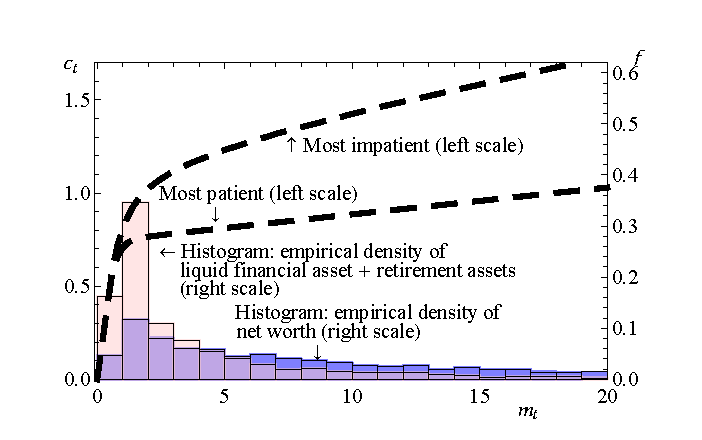
\includegraphics[width=0.8\textwidth]{../Figures/CFuncDistSevenPermAndHistNetWorthLiqFinPlsRetPlot.pdf}
\end{figure}
{\footnotesize Liquid Assets $\equiv$ transaction accounts,
CDs, bonds, stocks, mutual funds}
\end{frame}


%_______________________________________
\begin{frame}
\frametitle{{Match Net Worth vs.\ Liquid Financial Assets
%\\
%MPC: 0.19 $\uparrow$ 0.68
}}

\begin{itemize}
  \item Buffer stock saving driven by accumulation of \jemph{liquidity}
  \item May make more sense to match liquid (and retirement) assets\\ (\citet{hall:slump}, \citet{kvStim})
  \item \jemph{Aggregate MPC Increases Substantially: 0.23 $\uparrow$ 0.43}
\end{itemize}

\begin{footnotesize}
\begin{table}
\input ../Tables/MPCslidesLiqFinPlsRet.tex
\end{table}
\tiny{Notes: Annual MPC is calculated by $1-(1-$\text{quarterly MPC}$)^{4}$.}
\end{footnotesize}

\end{frame}





\begin{frame}[label=cfunc]
\frametitle{{Distribution of MPCs}}

{\jemph{Wealth heterogeneity translates into heterogeneity in MPCs}}

\begin{figure}
\centering
% 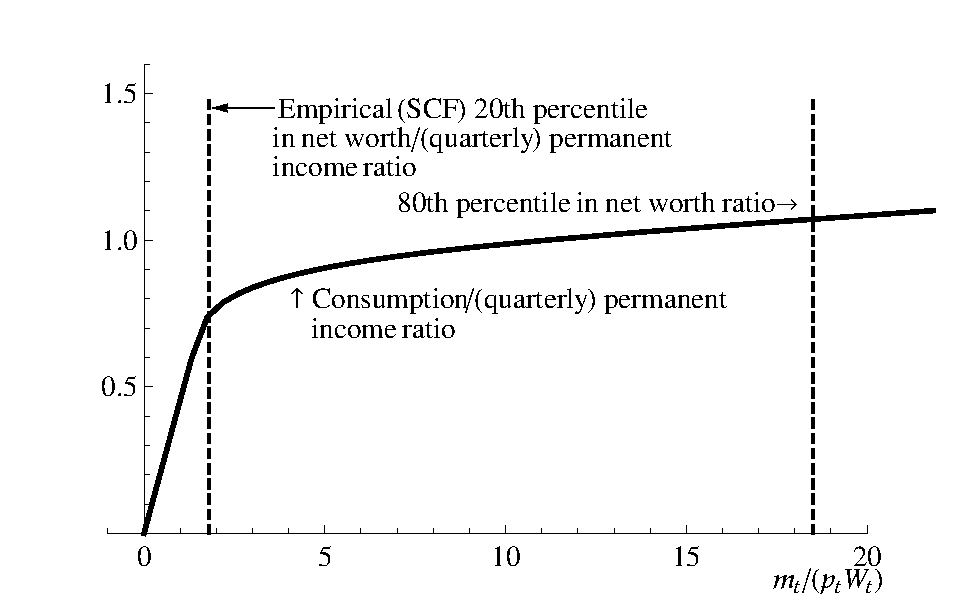
\includegraphics[width=\textwidth]{../Figures/CFuncPointPlotNW2080.pdf}
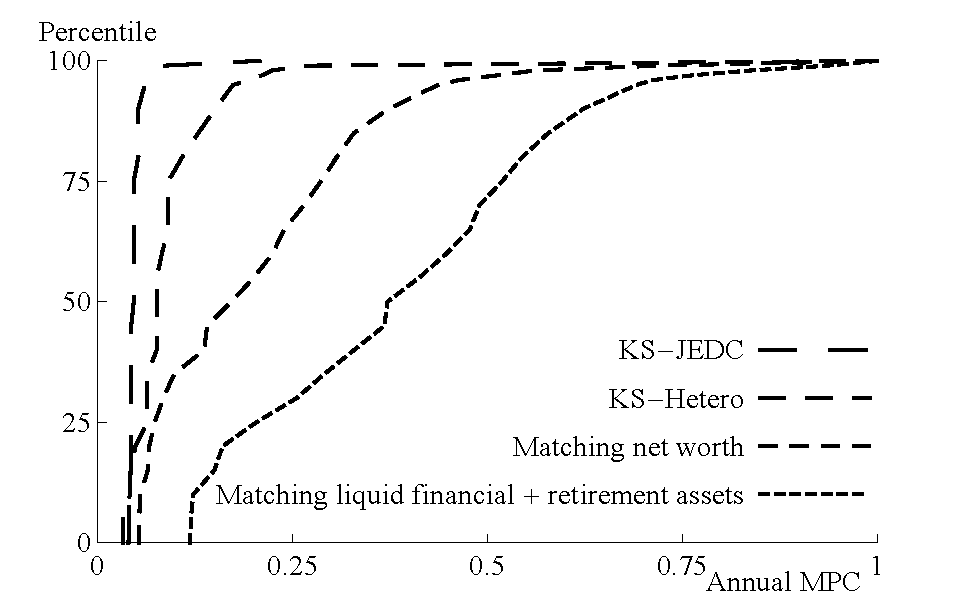
\includegraphics[width=0.8\textwidth]{../Figures/DistributionsMPCsDistSevenAndKSKSAggShocksPlot.pdf}

\end{figure}

\end{frame}



\begin{frame}
\frametitle{{Typology of Our Models---{Four Dimensions}}}

\begin{block}{}\footnotesize
\begin{enumerate}
\item<0-0> \jemph{Discount Factor $\Discount$}
\bi \scriptsize
\item \jemph{`$\Discount$-Point' model:} Single discount factor
\item \jemph{`$\Discount$-Dist' model:} Uniformly distributed discount factor
\ei
\item<0-0> \jemph{Aggregate Shocks}
\bi \scriptsize
\item (No)
\item Krusell--Smith
\item Friedman/Buffer Stock
\ei
\item<0-0> \jemph{Empirical Wealth Variable to Match}
\bi \scriptsize
\item Net Worth
\item Liquid Financial Assets
\ei
\item<1-> \jemph{Life Cycle}
\bi \scriptsize
\item Perpetual Youth (a la Blanchard)
\item Overlapping Generations
\ei
\end{enumerate}
\end{block}

\end{frame}


\section{Life Cycle Model}
\subsection{Overlapping Generations}
\begin{frame}
\frametitle{Dimension 4: Overlapping Generations}
\jemph{\textbf{Realistic Life-Cycle Model}}
\bi
\item Three education levels: $e\in\{D, HS, C\}$
\item Age/education-specific income profiles
\begin{eqnarray*}
\yLev_t &=& \tshk_t \pLev_t = (1 - \tau)\theta_t \pLev_t,\\
\pLev_t &=& \pshk_t \overline{\pshk}_{es} \pLev_{t-1}
\end{eqnarray*}
\bi
\item Age-specific variances of income shocks
\item Transitory unemployment shock with prob $\urate$
\ei
\item Household-specific mortality $\PDies_{es}$
\ei
\end{frame}

\subsection{Household Decision Problem}

\begin{frame}
\frametitle{Household Decision Problem}
\begin{eqnarray*}
\vFunc_{es}(\mRat_t) &=& \max_{\cRat_t} \util %(\cRat_t) + \Discount \PLives_{es} \Ex_t \left[\pshk_{t+1}^{1-\CRRA} \vFunc_{es+1}(\mRat_{t+1})\right]\\
%\notag &\text{s.t.}&\\
%\aRat_t &=& \mRat_t - \cRat_t,\\
%\kRat_{t+1} &=& \aRat_t/\pshk_{t+1},\\
%\mRat_{t+1} &=& (\daleth +\rProd) \kRat_{t+1} + \tshk_{t+1},\\
%\aRat_t &\geq& 0
\end{eqnarray*}
\end{frame}

\subsection{Macro Dynamics}
\begin{frame}
\frametitle{Macro Dynamics}
\bi
\item Population growth $N$, technological progress $\Gamma$
\item \jemph{Tax rate} to finance social security and unemployment benefits: $\tau=\tau_{SS}+\tau_U$
\item
$
\tau_{SS} = \frac{\sum_{e \in \{D,HS,C\}} \Big[ \theta_e \overline{\pLev}_{e0} \sum_{t = 164}^{384} \big( ((1 + \Gamma)(1+N))^{-t} \prod_{s=0}^t ( \overline{\pshk}_{es} \PLives_{es} ) \big) \Big]}
{\sum_{e \in \{D,HS,C\}} \Big[ \theta_e \overline{\pLev}_{e0} \sum_{t = 0}^{163} \big( ((1 + \Gamma)(1+N) )^{-t} \prod_{s=0}^t ( \overline{\pshk}_{es} \PLives_{es} ) \big) \Big]}
$
\item $\tau_U=\urate\mu$
\ei
\end{frame}

\subsection{Calibration}
\begin{frame}
\frametitle{Calibration}

\begin{table}
\footnotesize
\label{table:ParametersLifeCycle}
\begin{center}
\begin{tabular}{l c c}
\toprule
Description & Parameter & Value \\
\midrule
Coefficient of relative risk aversion & \CRRA & 1 \\
Effective interest rate & $(\rProd - \delta)$ & 0.01 \\
Population growth rate & $N$ & 0.0025 \\
Technological growth rate & $\Gamma$ & 0.0037 \\
Rate of high school dropouts & $\theta_D$ & 0.11 \\
Rate of high school graduates & $\theta_{HS}$ & 0.55 \\
Rate of college graduates & $\theta_C$ & 0.34 \\
Average initial permanent income, dropout & $\overline{\pLev}_{D0}$ & 5000 \\
Average initial permanent income, high school & $\overline{\pLev}_{HS0}$ & 7500 \\
Average initial permanent income, college & $\overline{\pLev}_{C0}$ & 12000 \\
Unemployment insurance payment & $\mu$ & 0.15 \\
Unemployment rate & $\urate$ & 0.07 \\
Labor income tax rate & $\tau$ & 0.0942 \\
\bottomrule
\end{tabular}
\end{center}
\end{table}

\end{frame}


\subsection{Results}
\begin{frame}
\frametitle{Results: Wealth Distribution}

\begin{figure}
\centering
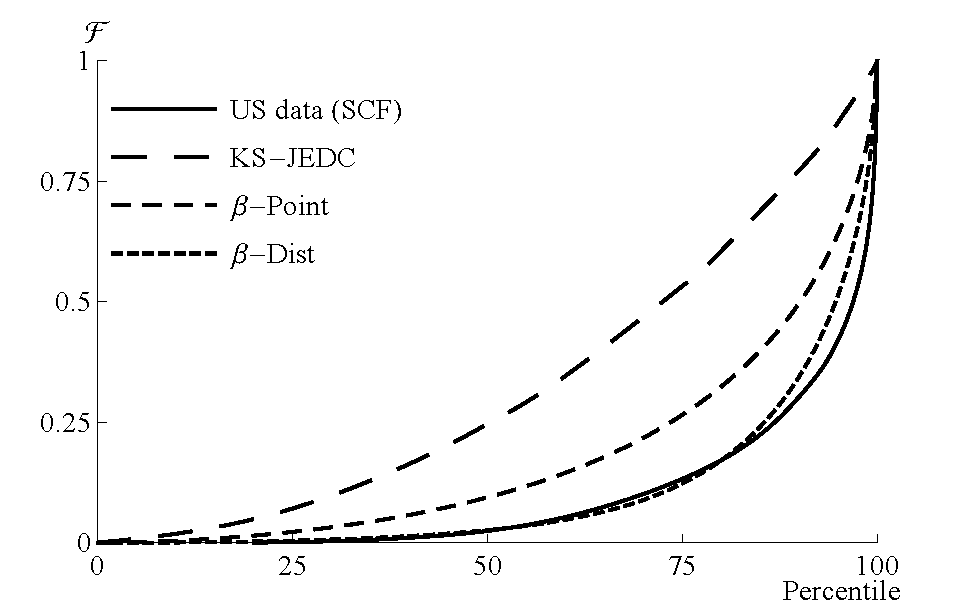
\includegraphics[width=0.9\textwidth]{../Figures/LifeCycleLorenzPlot.pdf}
%\caption{Cumulative Distribution of Net Worth}
\label{LifeCycleLorenzPlot}
\end{figure}

\end{frame}

\begin{frame}
\frametitle{{Results: MPC (in Annual Terms)}}
\begin{scriptsize}
\begin{table}
\input ../Tables/MPCslides_LCM.tex
\end{table}
\tiny{Notes: Annual MPC is calculated by $1-(1-$\text{quarterly MPC}$)^{4}$.
% See the paper for a discussion of the extensive literature that generally estimates empirical MPC's in the range of 0.3--0.6.
}
\end{scriptsize}
\end{frame}



\begin{frame}
\frametitle{Results: MPC by Age}

\begin{figure}
\centering
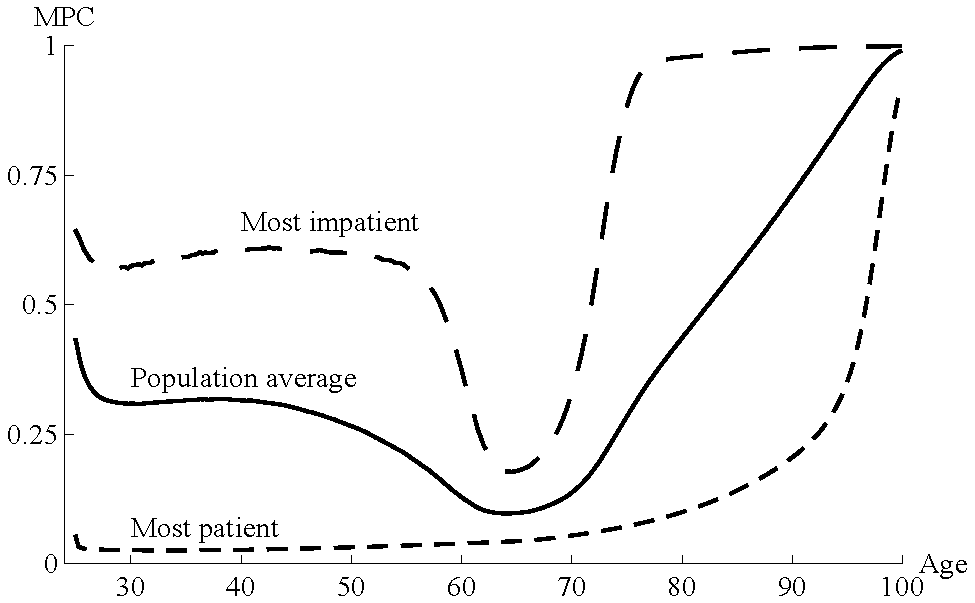
\includegraphics[width=0.7\textwidth]{../Figures/MPCbyAgeFigure.pdf}
%\caption{Cumulative Distribution of Net Worth}
\label{LifeCycleLorenzPlotByAge}
\end{figure}

\bi \scriptsize
\item Initial drop in MPC: Build-up of buffer stock
\item Rise while rapid income growth, fall before retirement, then incrsing mortlty risk
\ei

\end{frame}

%\section{Conclusions}
%_______________________________________
\begin{frame}
\frametitle{{Conclusions}}
\begin{itemize}
  \item Definition of ``serious'' microfoundations: Model that matches
\bi
\item Income Dynamics
\item Wealth Distribution
\ei
  \item The model produces more plausible implications about:
  \bi
  \item \jemph{Aggregate MPC}
  \item \jemph{Distribution of MPC Across Households}
  \ei
  \item Version with more plausible aggregate specification is\\
  \jemph{simpler, faster, better in every way!}
\end{itemize}
\end{frame}



%_______________________________________
%\renewcommand{\bibsection}{\subsubsection*{\bibname }}

%\nocite{denhaan:modelb}
\nocite{castaneda}


\beamerdefaultoverlayspecification{<*>}

\begin{frame}[allowframebreaks]
\frametitle{{References}}
\tiny
\input econtexBibMake
\end{frame}

